\documentclass{article}

\usepackage[english]{babel}
\usepackage[utf8]{inputenc}
\usepackage{amsmath,amssymb}
\usepackage{parskip}
\usepackage{graphicx}
\usepackage{listings}
\usepackage{float}
\lstset{
    numbers=left, 
    numberstyle= \tiny, 
    keywordstyle= \color{ blue!70},
    commentstyle= \color{red!50!green!50!blue!50}, 
    frame=shadowbox, % 阴影效果
    rulesepcolor= \color{ red!20!green!20!blue!20} ,
    escapeinside=``, % 英文分号中可写入中文
    xleftmargin=2em,xrightmargin=2em, aboveskip=1em,
    framexleftmargin=2em,
    breaklines=true,
    language=python
} 
% Margins
\usepackage[top=2.5cm, left=3cm, right=3cm, bottom=4.0cm]{geometry}
% Colour table cells
\usepackage[table]{xcolor}

% Get larger line spacing in table
\newcommand{\tablespace}{\\[1.25mm]}
\newcommand\Tstrut{\rule{0pt}{2.6ex}}         % = `top' strut
\newcommand\tstrut{\rule{0pt}{2.0ex}}         % = `top' strut
\newcommand\Bstrut{\rule[-0.9ex]{0pt}{0pt}}   % = `bottom' strut

%%%%%%%%%%%%%%%%%
%     Title     %
%%%%%%%%%%%%%%%%%
\title{CSCI803 Assignment}
\author{Yao Xiao \\ SID 2019180015}
\date{\today}

\begin{document}
\maketitle

%%%%%%%%%%%%%%%%%
%   Problem 1   %
%%%%%%%%%%%%%%%%%
\section{Problem 1}
\begin{figure}[H]
    \centering
    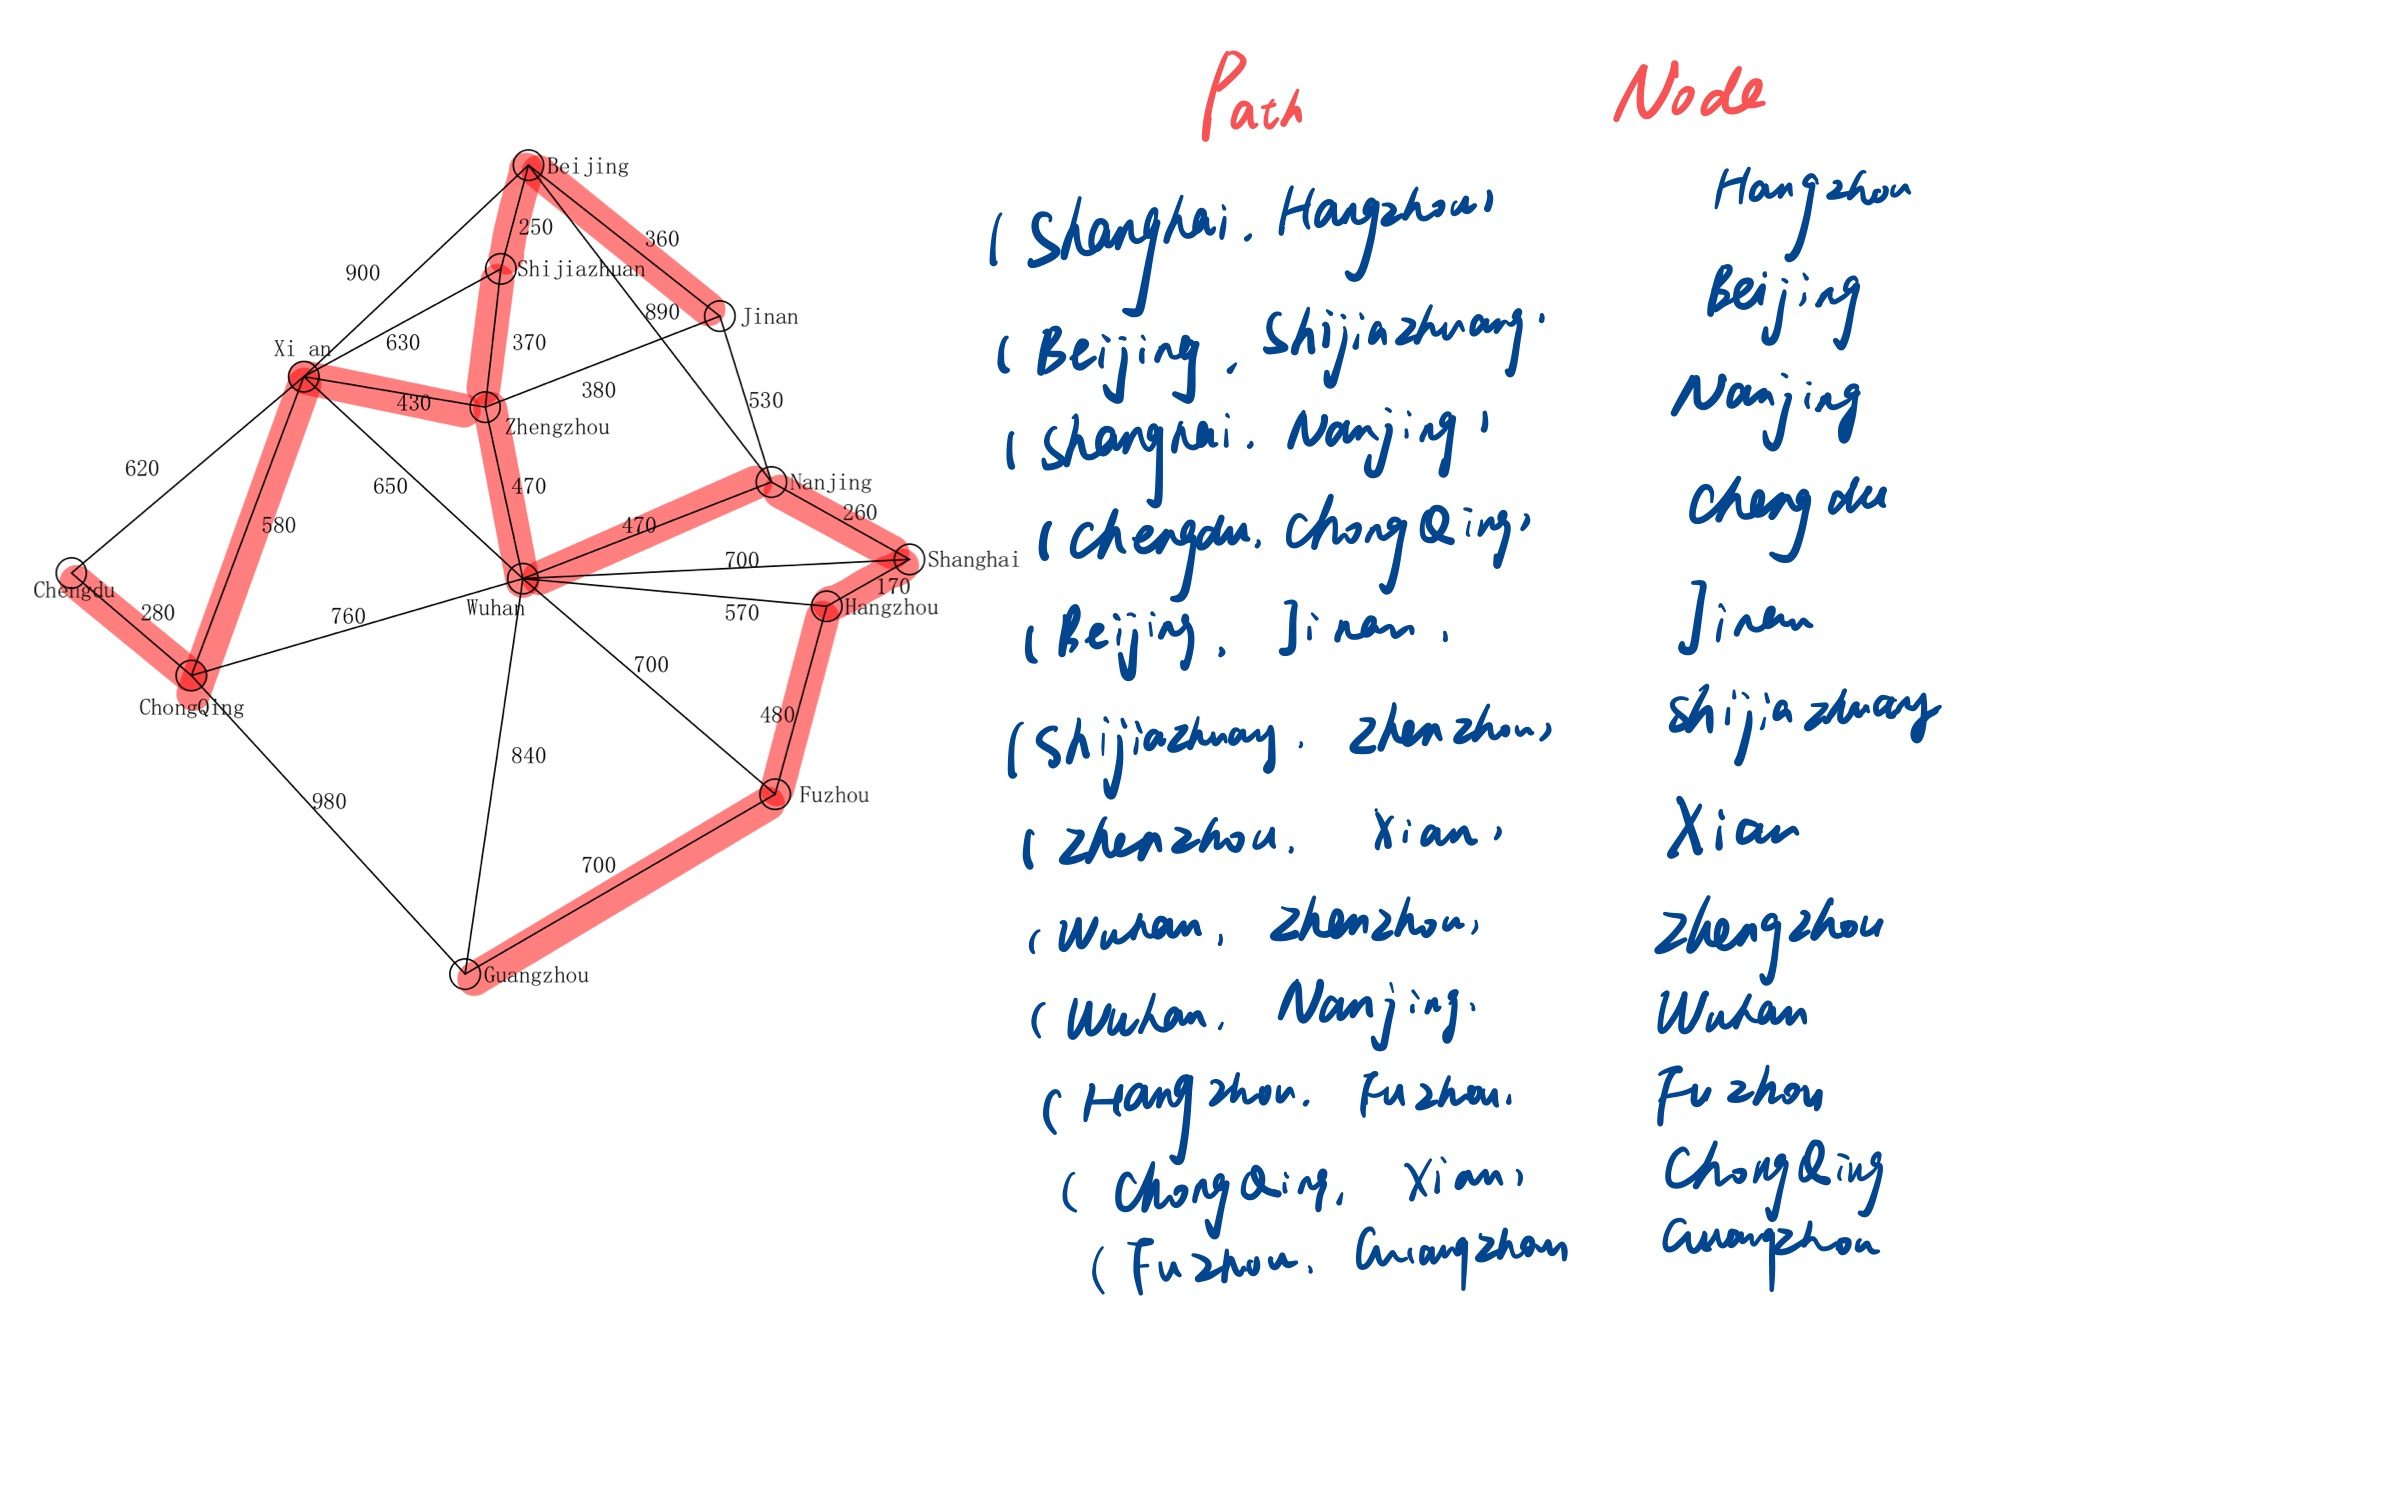
\includegraphics[width=1\textwidth]{Fig1}
\end{figure}


\section{Problem 2}
\begin{figure}[H]
    \centering
    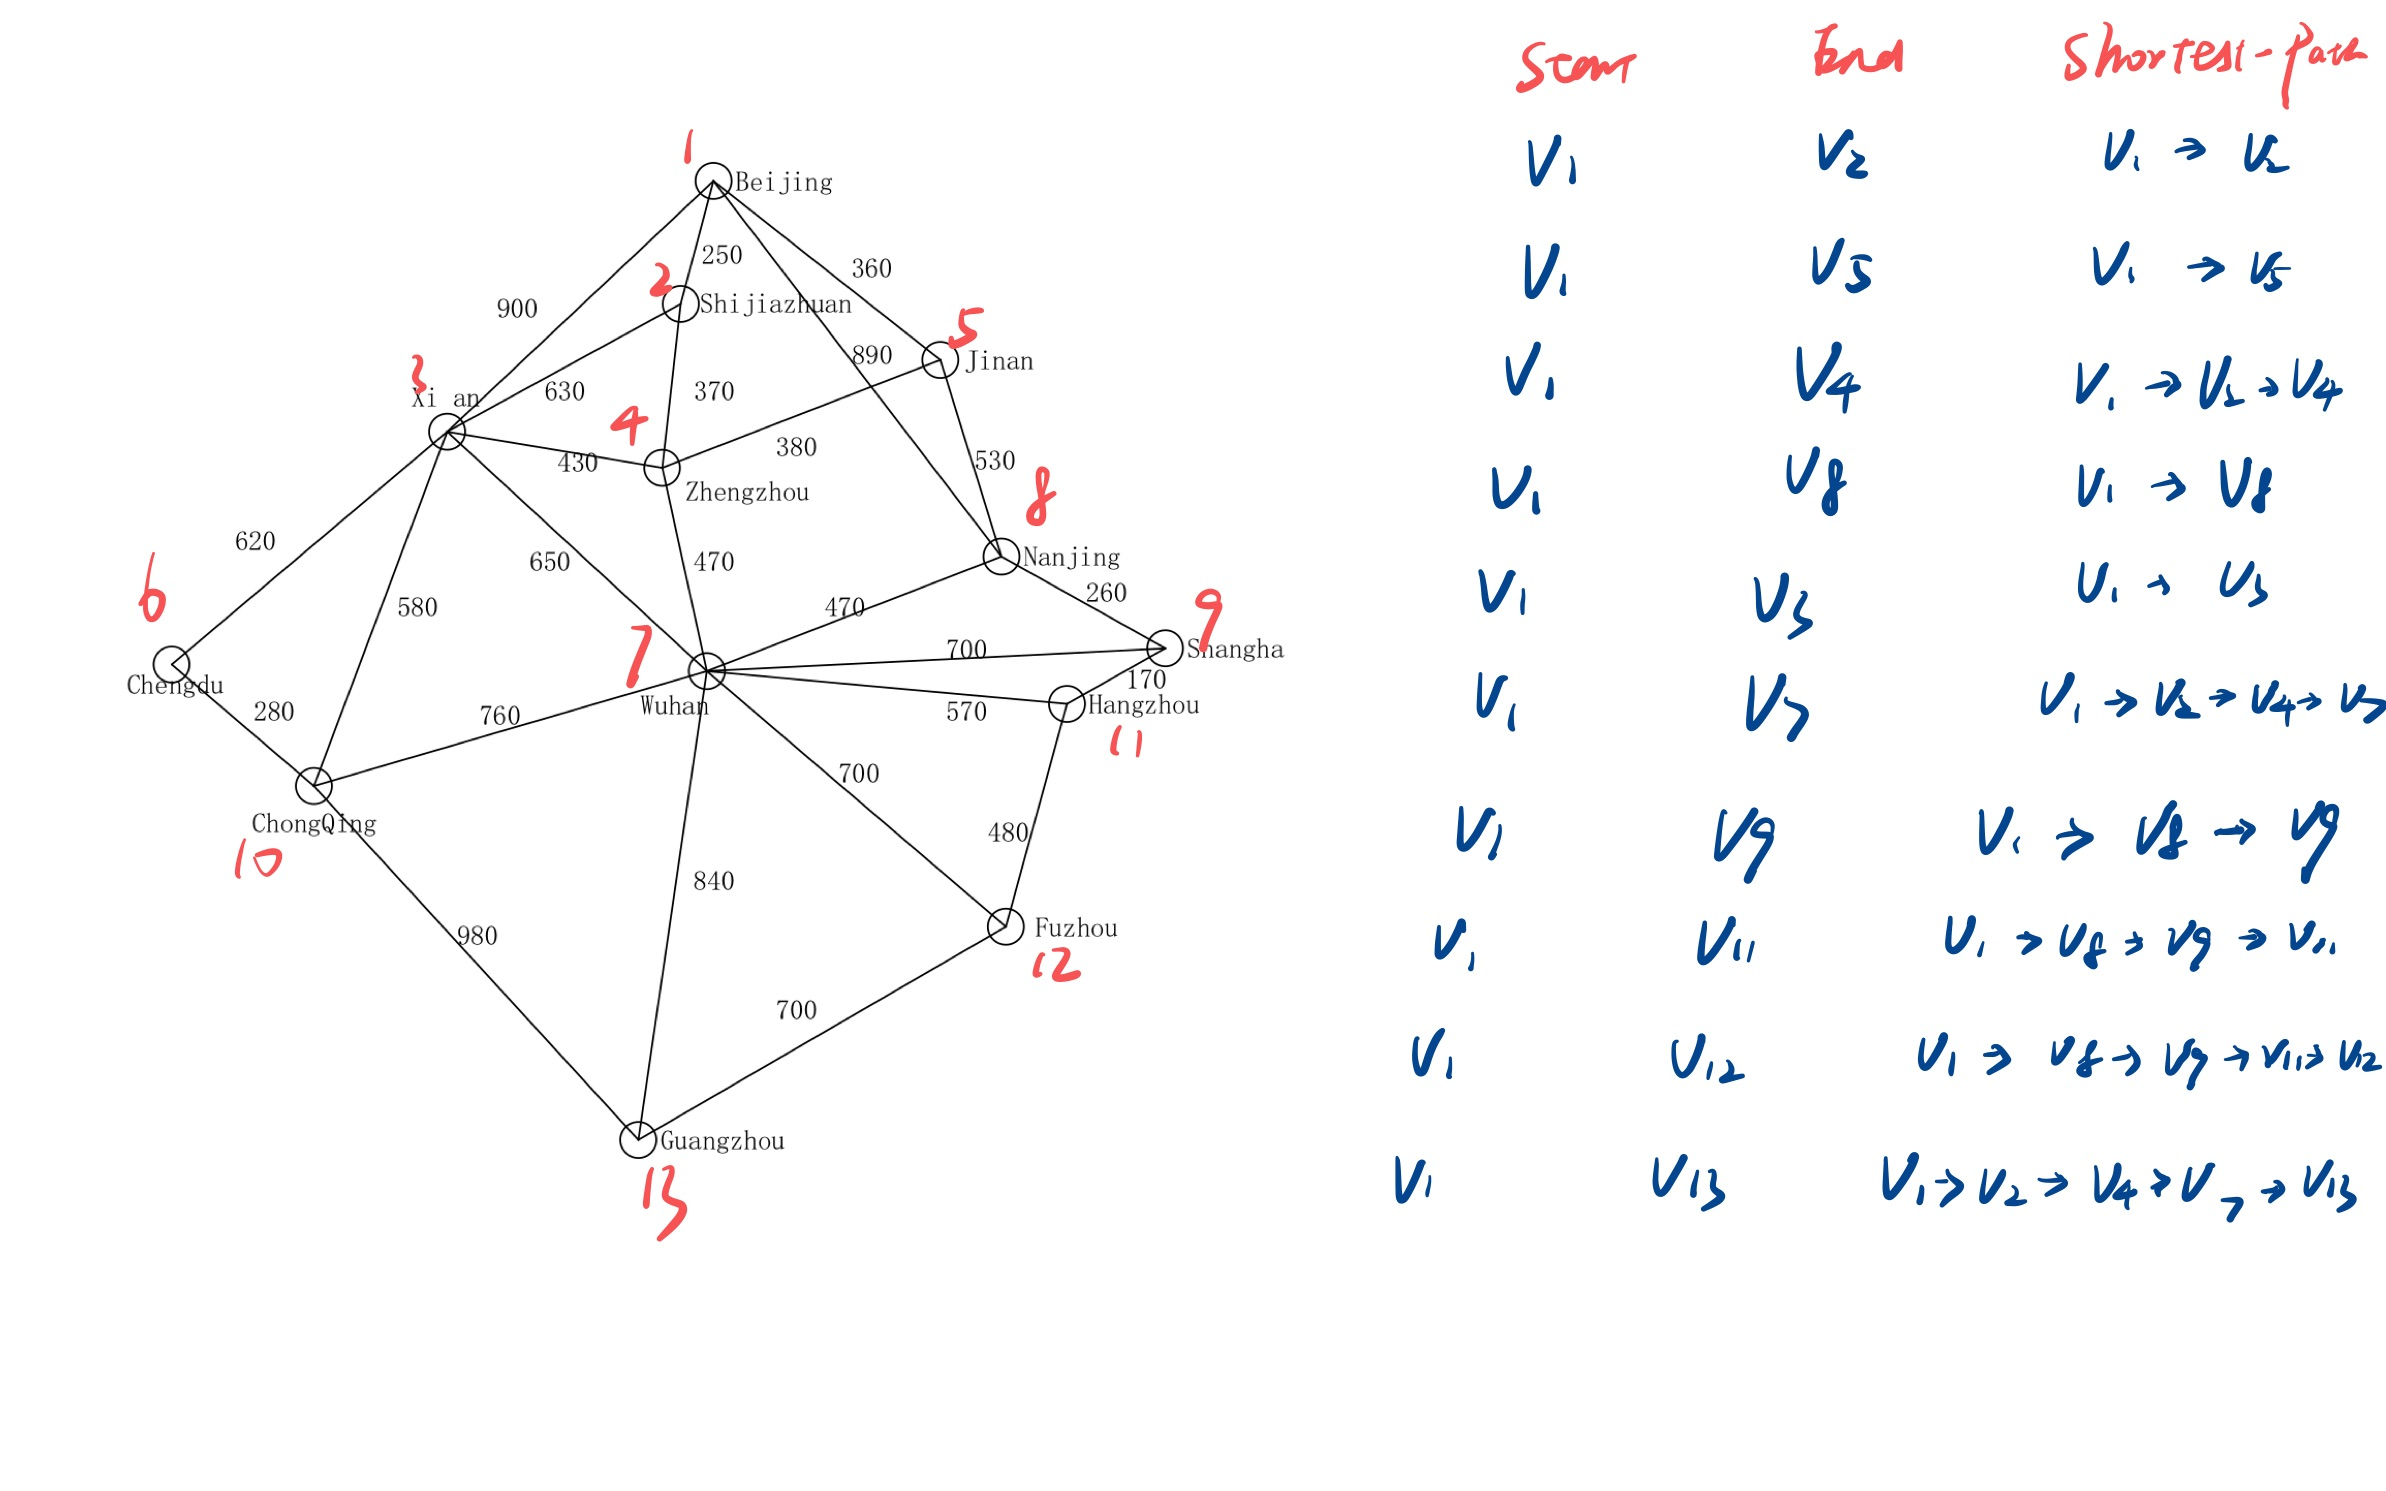
\includegraphics[width=1\textwidth]{Fig2}
\end{figure}

\section{Problem 3}
\begin{lstlisting}
from sys import argv
import re

great_node = -1
graph = []
file = open(argv[1], "r")

for line in file:
    if not re.match("//", line):
        info = line.split(" ")
        arrest = {info[0] + "&" + info[1]: info[2].replace('\n', '')}
        if int(info[0]) > great_node:
            great_node = int(info[0])
        if int(info[1]) > great_node:
            great_node = int(info[1])
        graph.append(arrest)

nodes = great_node + 1
prim = []
min_dist = {}
added = []
added.append(int(list(graph[0].keys())[0].split("&")[0]))

i = 0
while i < nodes:
    for node in range(len(graph)):
        n = list(graph[node].keys())[0].split("&")
        if (int(n[0]) in added or int(n[1]) in added) and (int(
                n[0]) not in added or int(n[1]) not in added):
            if len(min_dist) == 0:
                min_dist = graph[node]
            elif int(list(graph[node].values())[0]) < int(
                    list(min_dist.values())[0]):
                min_dist = graph[node]
    if min_dist:
        prim.append(min_dist)
        if int(list(min_dist.keys())[0].split("&")[0]) not in added:
            added.append(int(list(min_dist.keys())[0].split("&")[0]))

        if int(list(min_dist.keys())[0].split("&")[1]) not in added:
            added.append(int(list(min_dist.keys())[0].split("&")[1]))
    min_dist = {}
    i += 1


print("======MST Nodes=====")
print(prim)
print("======Final Cost=====")
cost = 0
for i in prim:
    if i:
        cost += int(list(i.values())[0])
print(cost)
\end{lstlisting}


\begin{figure}[H]
    \centering
    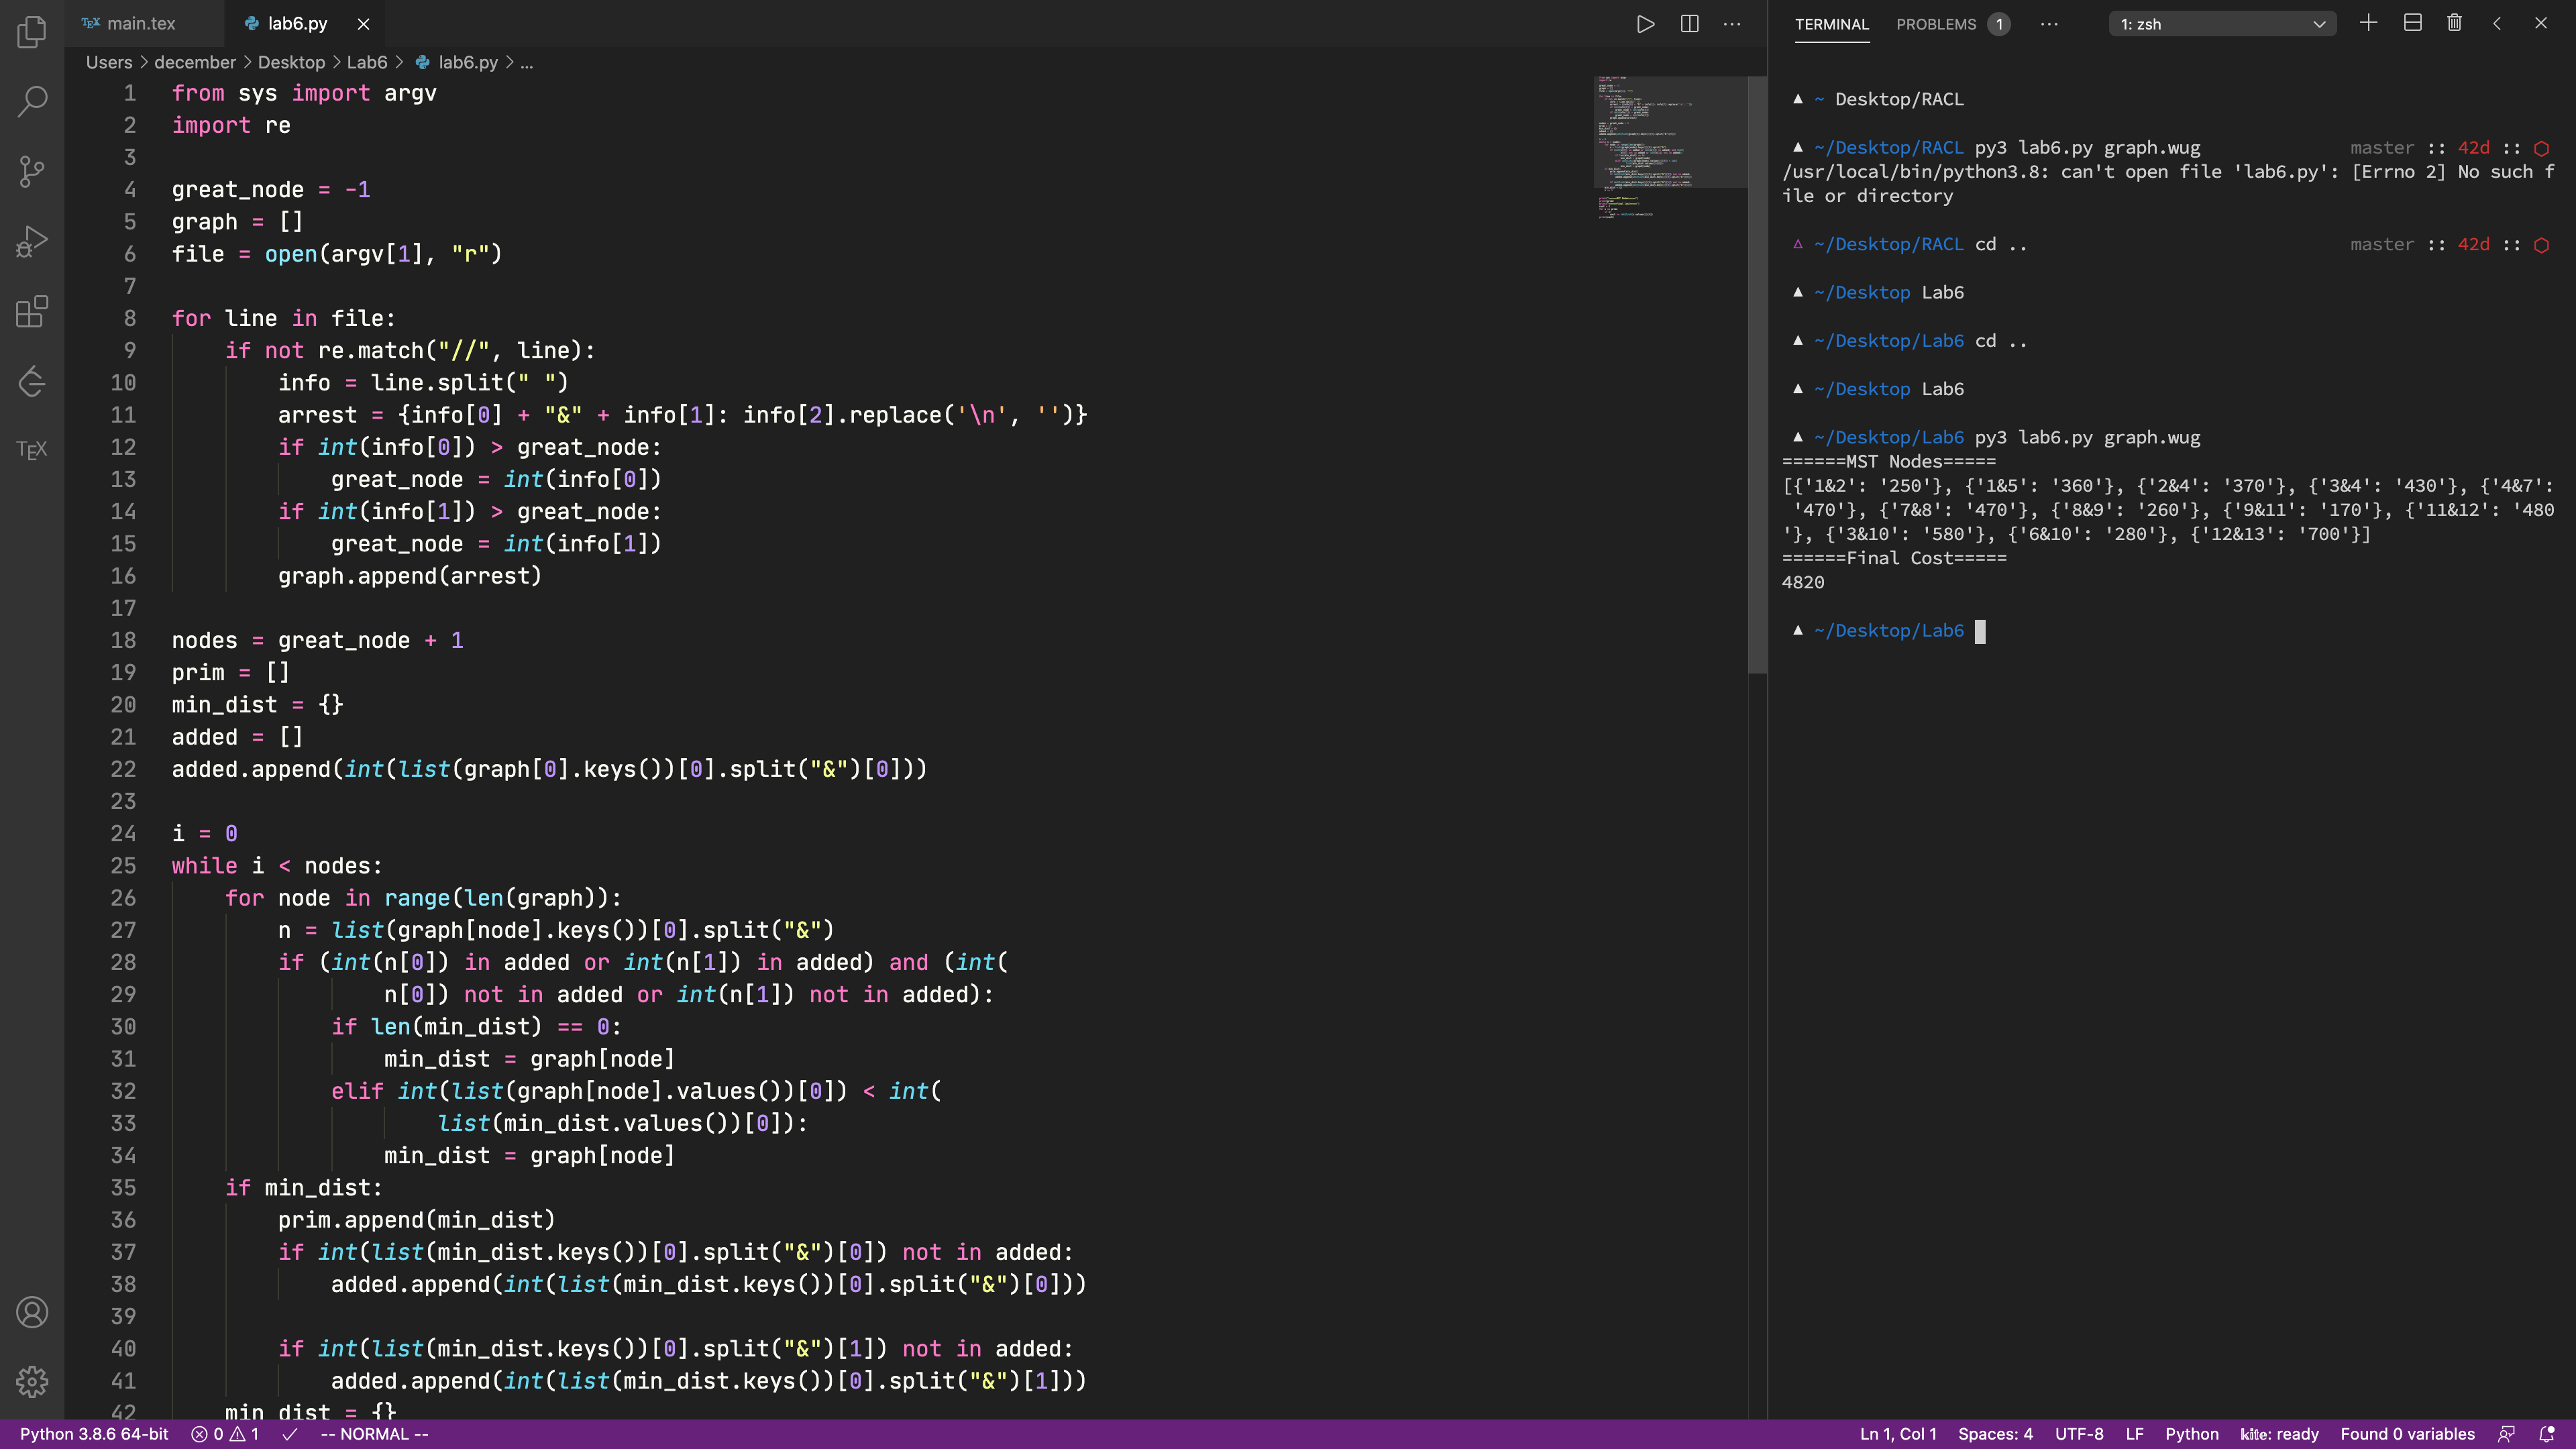
\includegraphics[width=1\textwidth]{Fig3}
\end{figure}




\end{document}
